\chapter{The LHCb Detector at the LHC}
\label{chap:detector}
%\chapquote{Teamwork is essential. It allows you to blame someone else.}{Finagle's Rule.}
The \lhcb experiment is one of the four major \gls{hep} experiments at the Large Hadron Collider (\lhc) and understands its primary focus in the realm of \bquark- and \cquark-physics.
The  \lhc is a particle accelerator located at the \cern facility.
Its main component is a storage ring with a total length of \SI{26.7}{\kilo\meter} in which protons are collided symmetrically.
At the time of writing the \lhc is the most powerful particle accelerator in the world.\footnote{Although powerful, it will most likely not destroy earth~\cite{lhcdestroyworld1,lhcdestroyworld2}.}
Since the year 2011, the proton beam energy has increased from \SI{3.5}{\tera\electron\volt} to \SI{4}{\tera\electron\volt} in the year 2012 and to \SI{6.5}{\tera\electron\volt} in the year 2015.
The periods of data taking are divided into the so-called \gls{runone} and \gls{runtwo} where the former refers to the years 2011 and 2012 and the latter to the years 2015 until 2018, corresponding to and integrated luminosity of roughly 3\,\invfb and 6\,\invfb, respectively.

Due to the large center-of-mass energy at the \lhc the highly correlated \bquark- and \bquarkbar-hadrons are predominately produced in the same forward or backward cone.
The \lhcb detector is thus designed as a (single arm) forward spectrometer, covering a forward cone from \SI{15}{\mrad} to \SI{300}{\mrad} in the bending plane and \SI{15}{\mrad} to \SI{250}{\mrad} in the non-bending plane.
The detector configuration consists of several tracking stations and calorimeters to reconstruct charged and neutral particles.
An effective particle identification is provided by a large dipole magnet and two Cherenkov radiators.
Different stages of hard- and software triggers reduce the event rate to a frequency at which events can be stored to disks.

In the present analysis we analyze the full available \gls{runtwo} dataset, recorded in the years 2015 until 2018.
Data recorded during the years 2011 and 2012 (\gls{runone}) are not taken into account for several reasons: First, from a technical point of view the experimental setup was frequently changed during \gls{runone}.
This includes changes to the trigger configuration which would require a separate analysis of data recorded during 2011 and the first and second half of 2012.
Secondly, only the second half of 2012 includes an efficient dedicated \Lz trigger, diminishing the total selection efficiency of the previous parts.
Thirdly, even though the \Lb production fraction is larger at small energies, this advantage is overcompensated by far due to the smaller \bbbar cross-section, making \gls{runtwo} significantly more efficient in terms of the overall signal efficiency.
Taking into account the larger data sample in terms of luminosity we conclude that adding \gls{runone} data could not help to significantly improve our results, but would imply disproportionate larger complexity and is therefore disfavored.

\section{Experimental Setup}
In the following we give a short overview about a selection of detector components that are relevant for the present analysis.
More detailed information, illustrations and thorough descriptions of the entire detector can be found in Refs.~\cite{lhcbdet,lhcbPerformance_run1}.
\begin{figure}[htbp]
    \centering
    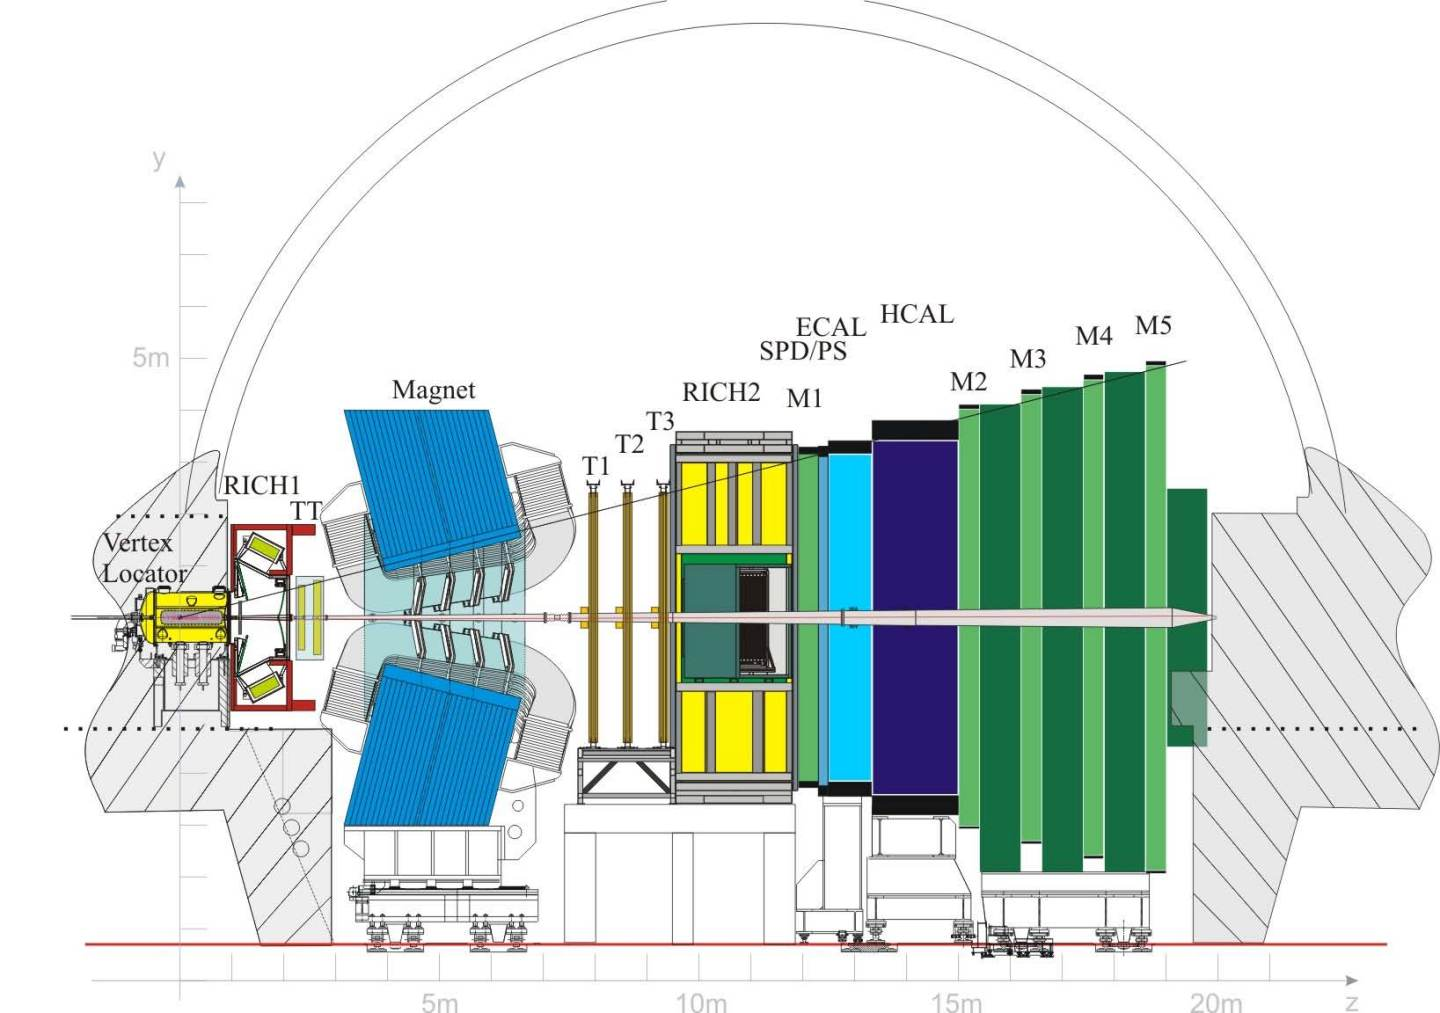
\includegraphics[width=.8\textwidth]{misc/lhcb_detector.png}
    \caption{Schematic view of the \lhcb detector by R.~Lindner (2008).}
\end{figure}

\subsection{Tracking}
\label{sec:detector_tracking}
A vertex locator (\gls{velo}) provides the precise measurements of tracks near of the \proton\proton interaction point.
Besides track reconstruction this information is also useful to distinguish primary vertices (\gls{pv}), \eg{}, from particles originating directly from the interaction point, and secondary vertices from long living \bquark- and \cquark-hadrons.
The \gls{velo} consists of \num{42} silicon modules, each of them equipped with radial and azimuthal strips.
The modules are semicircularly shaped and arranged in pairs such that they surround the beam pipe perpendicularly.
The pitches of the silicon sensors increase linearly from \SI{38}{\micro\meter} at the inner radius ($r=\SI{8.2}{\milli\meter}$) to \SI{102}{\micro\meter} at the outer radius ($r=\SI{42}{\milli\meter}$).
The spatial design of the modules was chosen such that charged particles with a pseudo rapidity $1.6 < \eta < 4.9$ cause at least three hits inside the \gls{velo}.
The total length of the \gls{velo} is not sufficient to cover all end vertices of long living $\PV^0$ particles such as the \Lz baryon or the \KS meson.
If both daughters of a $\PV^0$ two-body decay are reconstructed within the \gls{velo} we refer to the reconstructed tracks as long tracks (\gls{LL}).
Otherwise, if the reconstruction is only based on hits in the tracking stations TT and T1-T3, we refer to them as downstream tracks (\gls{DD}).
For the sake of brevity, we categorize entire decays chains, such as \decay{\Lb}{\Dz\Lz}, also as \gls{LL} (\gls{DD}) if both \Lz daughters are reconstructed as long (downstream) tracks.

Besides the \gls{velo}, four more tracking systems are placed, referred to as the TT, located upstream, and the modules T1, T2 and T3, located downstream of the spectrometer magnet.
The TT and the inner parts of the T1-T3 stations are constructed from p-on-n silicon microstrips detectors with a hit efficiency above 99\,\% and a hit resolution of approximately \SI{50}{\micro\meter}.
%The TT is \SI{150}{\centi\meter} wide and \SI{130}{\centi\meter} high.
The silicon microstrips are arranged in four layers, corresponding to an active area of approximately \SI{8}{\meter\squared}.
The resolution of the T1-T3 stations varies from the innermost towards the outer parts.
Whereas silicon strips are used for the inner parts, the outer parts of the T1-T3 stations are straw-tubes.
The straw-tubes measure the drift time of ionised charges with a total delay below \SI{75}{\nano\second}.

\subsection{Ring Imaging Cherenkov Detectors}
Two Ring Imaging Cherenkov detectors (\gls{rich}), referred to as RICH1 and RICH2, detect Cherenkov light.
Cherenkov radiation is an electromagnetic radiation that gets emitted by charged particles in a dielectric medium if the velocity $v$ of the particles is greater than the (group) velocity $c_m$ of the given medium.
For constant velocities the emitted light cone has a constant opening angle $\phi$,
\begin{equation*}
    \sin \frac{\phi}{2} = \frac{c_m}{v} = \frac{c_0}{nv} \,,
\end{equation*}
and thus directly allows the inference of $v$ if the refractive index $n$ (and the speed of light in vacuum $c_0$) is known.
Inside the \gls{rich} units, Cherenkov cones are mapped to spherical coordinates $(r,\vartheta)$, where $r$ is a function of the opening angle $\phi$ and $\vartheta$ is the azimuthal part of the Cherenkov photons trajectory.
This projection is achieved via spherical mirrors which reflect the photons to Hybrid Photon Detectors where they are detected.
By combining the measurements of the opening angle $\phi$ as a function of $v$ and the deflection in the magnetic field, a hypothesis for the invariant mass can be set and thus allow to identify the particle (\cf{} Sec.~\ref{sec:detector_pid}).
%Although vacuum could be used as a radiator in theory~\cite{vacuumcherenkov}, each \gls{rich} unit is filled with a different gas admixture, corresponding to different refractive indices to lower the Cherenkov thresholds and to allow a diverse momentum resolution.
Each \gls{rich} unit is filled with a different gas admixture, corresponding to different refractive indices to lower the Cherenkov thresholds and to allow a diverse momentum resolution.
Since \gls{runtwo}, RICH1 is filled with $\mathrm{C}_4\mathrm{F}_{10}$, whereas $\mathrm{CF}_4$ is used as the radiator in RICH2, making the units sensitive to the momentum ranges $2$ to $60\,\gevc$ and $15$ to $100\,\gevc$, respectively. (Particle dependent thresholds are listed in Tab.~\ref{tab:rich_thresholds}.)

\subsection{Calorimeters}
Neutral particles like photons are neither deflected in magnetic fields, nor do they emit Cherenkov light, nor are they detected in the \gls{velo}, TT and T1-T3, hence a calorimeter system is necessary.
The calorimeters bring a large amount of material into the detector as they have to stop the passing particles completely to measure the deposited energy.
In order to not affect the measurements in the tracking stations, they are placed downstream of them.
In total, four types of calorimeters are used in the \lhcb detector.
Together they provide the identification of electrons, protons and other hadrons, as well as the energies and positions of photons and neutral hadrons.
Furthermore, the calorimeter measurements are used to select candidates with high transverse momentum for the first trigger level \gls{lzero}.
The four calorimeter systems are a scintillating pad detector (\spd), a preshower calorimeter (\presh), an electromagnetic calorimeter (\ecal) and an hadronic calorimeter (\hcal).
The first two systems consist of plain scintillator tiles, separated from each other by a thin lead layer (2.5 radiation lengths), and the \ecal (25 radiation lenghts) and \hcal systems have a shashlik\footnote{A sampling scintillator and lead structure perpendicular to the beam axis.} and a sampling construction\footnote{A sampling scinitillator and iron structure parallel to the beam axis.}, respectively.
During the traversal, the particles are stopped in the lead and iron layers and deposit their energy.
This energy produces light in the (organic) scintillators which is transmitted via optical fibers to photo multipliers where the photons are detected.
Since the hit density varies over the calorimeter surface perpendicular to the beam axis, a variable lateral segmentation is adopted.
The outer dimension is chosen such that it projectively matches those of the tracking system and the inner dimension is limited by the beam pipe.
During \gls{runtwo}, the \ecal and \hcal are predominantly used for contributing to the trigger decisions, \cf{}~Sec.~\ref{sec:detector_trigger}.

\subsection{Muon System}
Although muons are charged particles their interaction is small compared to hadrons like pions or kaons due to their leptonic nature, and also small to the electron due their large invariant mass.
Muons thus do not deposit their entire energies in the calorimeters and dedicated muon systems are necessary.
In total, five rectangular shaped muon stations M1-M5 are placed up- and downstream of the calorimeter systems.
M1 is a triple gas electron multiplier and is placed upstream in front of the calorimeter stations in order to improve measurements of the transverse momentum within the trigger logic.
The stations M2-M5 are multi wire proportional chambers and are placed downstream behind all other detector units.
In order to discriminate muons against the abundant hadronic background and cosmic rays, muons are required to produce aligned hits in all five stations, corresponding to a minimum momentum above $6\,\gevc$.
The stations are interleaved by thick iron absorbers of 20 nuclear interaction lengths.
The chambers cover an active area of \SI{435}{\meter\squared}, have a time resolution below \SI{4.5}{\nano\second} and differ in their lateral segmentation similar to the tracking stations and the calorimeter systems.

\subsection{Dipole Magnet}
The spectrometer magnet is a warm dipole magnet with a saddle-shaped coil design in a window frame yoke with sloping poles.
It provides an integrated magnet field of roughly \SI{4}{\tesla\meter} for particles with a track length of \SI{10}{\meter}.
Three smaller dipole magnets inside this magnet compensate the impact on the \lhc beam.
In order to analyze and cancel asymmetries of the detector units between oppositely charged tracks, the polarity of the magnetic field can be switched.
In the following we refer to these states as \textit{mag.\ up} and \textit{mag.\ down}.
Unfortunately, the magnetic field is not known exactly throughout the entire detector (neither temporal, nor spatial), thus leading to an inexact calibration of the particle momenta.
Furthermore, charged particles loose energy by ionization or by emitting photons when they traverse material or are deflected in a magnet field.
The emitted particles (typically electrons or photons) tend to have low energies and therefore remain undetected.
Such losses are only reproduced partially in simulations, hence the reconstructed energy of particles is too low, resulting in asymmetries in the inferred momenta.
Additionally, misalignment effects of the detector units lower the resolution.

Software tools are available that mitigate these effects by correcting the momentum scale phenomenological.
During the present analysis we use a tool which calibrates the scale with the two-body decays \decay{\jpsi}{\mup\mun} and \decay{\Bd}{\jpsi\Kp} where in the former the dimuon pair and in the latter the \Kp is used for the calibration.
The samples are split w.r.t.\ the product of particle charge and magnet polarity and thus removes a potential bias due to whether the particles are deflected inwards or outwards by the magnet field.

\subsection{Trigger System}
\label{sec:detector_trigger}
The \lhc machine operates with a bunch crossing frequency of \SI{40}{\mega\hertz} which is unfeasible for any kind of unfiltered reconstruction or data storing.
A dedicated trigger system thus select bunch crossings with at least one inelastic $\proton\proton$ interaction and further reduces its rate below \SI{12.5}{\kilo\hertz} by applying filter criteria which, in general, aim to select \bquark- and \cquark-quark decays.
The trigger system is arranged in two different tiers, referred to as the low level trigger \gls{lzero} and the high level trigger \gls{hlt}.

The \gls{lzero} trigger is directly implemented in hardware and reduces the event rate below \SI{1.1}{\mega\hertz} by combining information of the calorimeters and the muon systems.
The complexity of \gls{lzero} decisions are strictly limited by the \lhc bunch crossing frequency and latency constraints, and allows only read-outs of the transverse energy deposited by showers in clusters in the calorimeter systems \spd, \presh, \ecal and \hcal, as well as transverse momenta measured in the muon chambers.

The trigger decision in the calorimeter is based on the transverse energy $E_T$ of single clusters where a cluster consists of $2 \times 2$ calorimeter cells.
The transverse energy of each cell $E_{T,i}$ is corrected by an inclination angle $\theta_i$ of a hypothetical neutral particle, accumulated,
\begin{equation*}
    E_T = \sum_{i=1}^4 E_{T,i} \sin \theta_i \,,
\end{equation*}
and tested against thresholds.
In particular, the \gls{lzero} decision for hadrons is based on single tracks and thus is insensitive to different decay topologies, \eg{}, \decay{\Lb}{\Dz\proton\pim} and \decay{\Lb}{\Dz(\decay{\Lz}{\proton\pim})} have a similar \gls{lzero} responses if the invariant mass of \proton \pim is close to $m(\Lz)$, whereas for \decay{\Lb}{\Dz\proton\pim} and \decay{\Lb}{\Dz\proton\Km} the \gls{lzero} response can vary due to different hadronic showers signatures of \pim and \Km.
Unlike the $E_T$ based decisions of showers in the calorimeters, the transverse momenta measured in the muon chambers does take combinations of up to two tracks into account and thus leverages an effective triggering of dimuon pairs for example in high statistics modes such as \decay{\Lb}{\jpsi\Lz}.

The \gls{lzero} trigger system rejects collisions for further processing if the transverse energy of clusters (calorimeter) or transverse momenta (muon chambers) are below certain thresholds.
The nominal value of each threshold is the objective of an online maximization of the signal efficiency under different \lhc conditions and are tuned during data taking.
\gls{mc} simulated events typically scale these thresholds and do not reflect temporal changes since this would imply an unnecessary waste of computing intensive detector simulations.
The fidelity of the \gls{lzero} trigger response in \gls{mc} simulated events thus has to be studied carefully if needed.

The latency of an individual \gls{lzero} decision is \SI{4}{\micro\second} which allows a subsequent read-out of the entire detector for the \gls{hlt} trigger which include a full off-line event reconstruction.
The \gls{hlt} was completely redesigned for the \gls{runtwo} data taking period due to changes of the bunch crossing frequency and the amount of visible interactions per bunch crossing, and now differs strongly from its previous design outlined in Ref.~\cite{lhcbDetector}.
During \gls{runtwo} the \gls{hlt} performs partial and full event reconstructions in software applications running on computing farms and stores the events at a rate of \SI{12.5}{\kilo\hertz}.
An in-depth description, as well as efficiency studies of the \lhcb trigger system can be found in Refs.~\cite{trigger11,trigger12} (\gls{lzero} and \gls{hlt} studies for \gls{runone}) and Ref.~\cite{triggerRun2} (\gls{lzero} and \gls{hlt} studies for \gls{runtwo}).

Terminology-wise, events of a decay directly involved in setting a trigger (line) are called \gls{tos} (trigger on signal) events.
If set, triggers typically cause the entire event to be stored to disk, including the decay tree initiated by the other associated \bquark- or \cquark-quark, even if not necessarily involved in the trigger decision.
These events are called \gls{tis} events (trigger independent of signal).
We note that both decay trees of a \bbbar or \ccbar pair can set trigger (lines).
In this case they are both considered \gls{tos} and \gls{tis}.

\subsection{PID}
\label{sec:detector_pid}
The particle identification (\gls{pid}) at \lhcb is built upon information of four different detector parts.
The calorimeters mainly contribute to the recognition and identification of neutral particles (\Pgamma, \piz) or electrons, muon chambers identify muons and the two \gls{rich} systems primarily identify charged hadrons (\pip, \pim, \Kp, \Km, \proton, \antiproton) and contribute to the identification of charged leptons (\electron, \muon) as well.

This information is gathered by two different approaches.
In the first method the likelihood information of each of the four subsystems is accumulated in a combined log-likelihood difference.
During analysis we refer to it as \gls{dll}, for example $\operatorname{\gls{dll}}(X-Y)$, where $X$ and $Y$ are two different mass hypotheses.
The second method utilizes a shallow neural network with the information of the four subsystems as the input layer, one hidden layer and six output neurons which are trained w.r.t.\ the particle hypotheses \electron, \muon, \kaon, \pion, \proton and \textit{ghost}, where the latter refers to trajectories that do not correspond to a single particle (\cf{}~\gls{ghostprob}).
These neural networks thus also encode correlations between the detector units and typically outperform the more canonical approach of linear adding log-likelihoods differences~\cite{lhcbPerformance_run1,lhcbDetector,lhcbmlpid}.
In the present analysis we refer to the numerical value of a neuron (output layer) corresponding to a particle hypothesis $X$ for a given particle $Y$ as $\texttt{ProbNNx}(Y)$.
The neurons are trained to yield large values if a given hypothesis is met, \eg{}, requiring large values for $\texttt{ProbNNk}(\proton)$ could be used as a veto against kaons for proton candidates.
The numerical value is normalized to the interval $[0,1]$ and is thus said to be interpretable as probabilities for the given particle hypothesis (hence the name).
We adopt the name but avoid the probability interpretation in the following.\footnote{This clearly depends on the given definition of \textit{probability}. Recent results show that the output of certain neural network can in fact be interpreted as probabilities via Bayesian inference~\cite{bayesnn1,bayesnn2}. However, the shallow networks used for \gls{pid} in the present analysis do not use such techniques.}

The \gls{pid} value of the \gls{rich} systems are based on $\operatorname{\gls{dll}}(X-Y)$ values where $X$ and $Y$ are two different mass hypotheses.
For the \gls{rich} to yield a meaningful number for this (i.e. not zero) it requires:
\begin{itemize}[itemsep=2pt,parsep=2pt]
    \item The track is in the acceptance of at least one of the two \gls{rich} radiator volumes.
    \item The expected signature in the \gls{rich} is different for $X$ and $Y$.
\end{itemize}
The former criterion does not change with the mass hypothesis assigned to a track, but depends dominantly on the path length of particles that traverse the \gls{rich} volumes.
The latter means that at least one of the two hypothesis $X$ or $Y$ (the lightest) needs to be above threshold, in at least one \gls{rich} radiator.
If one of $X$ or $Y$ is below threshold, that does not matter, as long as the other is above.
The momentum thresholds for different (charged) particles, calculated from the (measured) \gls{rich} refractive indices are given in Tab.~\ref{tab:rich_thresholds} below.
\begin{table}[htbp]
    \centering
    \caption{Momentum thresholds in \gevc of the RICH systems for different charged particles, calculated from the measured refractive indices of the RICH systems and the respective particle masses.}
    \label{tab:rich_thresholds}
    \begin{tabular}{lSS}
        \toprule
        Particle & {RICH1 [\gevc]} & {RICH2 [\gevc]} \\
        \midrule
        $\electron^\pm$ & 0.00978 & 0.0170 \\
        $\muon^\pm$ & 2.02 & 3.52 \\
        $\pion^\pm$ & 2.67 & 4.65 \\
        $\kaon^\pm$ & 9.45 & 16.4 \\
        $\proton$, $\antiproton$ & 17.9 & 31.3 \\
        $\Pd$, $\overline\Pd$ & 35.9 & 62.6 \\
        \bottomrule
    \end{tabular}
\end{table}

\section{Variables and Acronyms used as Selection Criteria}
\label{sec:selvar}
During analysis we frequently use abbreviations and acronyms which refer to variables that are used for discriminating background events.
Below, we give a short overview over the most common ones and occasionally refer to this list in the subsequent chapters.
\begin{description}
    \item[\dchisqip] Difference between the $\chi^2$ value of the \gls{pv} reconstructed with and without the track under consideration. Clearly, by adding an additional \gls{dof} the $\chi^2$ value will always improve, however the improvement is less pronounced for spurious than for genuine tracks on average.
    \item[\dll$(X-Y)$] Delta log-likelihood of \gls{pid} values of the \gls{rich} systems w.r.t.\ the different mass hypotheses $X$ and $Y$.
    \item[\dira] Cosine of the angle between the momentum of the particle and the direction vector from some reference vertex or 3D-point to the end-vertex of the particle.
    \item[\doca] Distance of closest approach for pairs of tracks. This quantity is evaluated before applying a \gls{dtf} since the latter forces this value to zero for all daughters of a common mother. In general, the \doca{} of the daughters of a (common) decay is small (albeit non-zero due to finite resolution effects) and large for random track combinations on average.
    \item[$|m(X) - \text{PDG}|$] The absolute difference between the invariant mass of particle \PX as obtained from four momentum addition and the respective nominal value (typically provided by the \gls{pdg}).
    \item[Best fit probability] If multiple \glspl{pv} are reconstructed for a single event the matching is ambiguous in \glspl{dtf} with constraint \gls{pv}. We disambiguate by choosing the \gls{pv} corresponding to the best fit in terms of the evaluated $\chi^2$ value and refer to it as the \textit{best} fit.
    \item[\Gls{ghostprob}] Output of a neural network based algorithm to identify tracks which do not correspond to the trajectory of a (single) true particle but rather originates from detector noise or multiple particles due to mismatching~\cite{ghostprob}.
%    \item[$\pt$] Magnitude of the component of particles three-momentum that is transverse to its flight direction. We note that this magnitude is a Lorentz invariant.
\end{description}
